\documentclass[conference]{IEEEtran}
\IEEEoverridecommandlockouts
% The preceding line is only needed to identify funding in the first footnote. If that is unneeded, please comment it out.
\usepackage{cite}
\usepackage{amsmath,amssymb,amsfonts}
\usepackage{algorithmic}
\usepackage{graphicx}
\usepackage{textcomp}
\usepackage{xcolor}
\def\BibTeX{{\rm B\kern-.05em{\sc i\kern-.025em b}\kern-.08em
    T\kern-.1667em\lower.7ex\hbox{E}\kern-.125emX}}
\begin{document}

\title{GPU-Only Neural Network Inference Using Fragment Shaders in OpenGL}

\author{
\IEEEauthorblockN{1\textsuperscript{st} Leanid Bintsarouski}
\IEEEauthorblockA{
\textit{Faculty of Applied Mathematics}\\
\textit{and Computer Science} \\
\textit{Belarusian State University}\\
Minsk, Belarus \\
binleo07@icloud.com
}
\and
\IEEEauthorblockN{2\textsuperscript{st} Dzianis Pirshtuk}
\IEEEauthorblockA{
\textit{Faculty of Applied Mathematics}\\
\textit{and Computer Science} \\
\textit{Belarusian State University}\\
Minsk, Belarus \\
ORCID: 0009-0009-7831-1953 \\
}
}

\maketitle

\begin{abstract}
This paper addresses the efficient use of neural networks on graphics processing units (GPUs). A GPU-only inference pipeline was designed and implemented using fragment shaders in OpenGL. The proposed solution avoids reliance on CPU interaction, allowing for real-time neural network execution on a wide range of devices, including mobile and embedded platforms. Performance was benchmarked against industry-standard frameworks such as TensorFlow Lite and MediaPipe. The results demonstrate that GPU shader-based inference can achieve competitive latency, with significantly reduced energy consumption and memory usage. This approach is applicable to fields such as augmented reality, automotive systems, and biomedical imaging.
\end{abstract}

\begin{IEEEkeywords}
neural networks, GPU, fragment shaders, OpenGL, real-time inference, TensorFlow Lite, MediaPipe, ESPCN
\end{IEEEkeywords}

\section{Introduction}
In recent years, there has been a marked increase in demand for high-performance and low-latency neural network execution on edge devices. Conventional CPU-based solutions frequently prove incapable of meeting real-time constraints or necessitate excessive power. Graphics processing units (GPUs) were originally developed for the purpose of rendering graphics. However, they have evolved into a potent substitute due to their massively parallel architecture.

This paper explores the potential of fragment shaders [5], which are commonly employed in rendering pipelines, for the purpose of neural network inference. In contrast to general-purpose compute APIs such as CUDA or Vulkan Compute, fragment shaders demonstrate a high level of platform support, encompassing mobile and embedded systems.

\section{Related Work}
Existing libraries such as TensorFlow Lite [1] and PyTorch Mobile [2] support GPU acceleration, yet still rely on CPU-GPU communication and intermediate memory copies. While the efficacy of this architecture is evident, it must be noted that it introduces latency and overhead.

A number of studies have been conducted on the utilisation of WebGL and OpenGL shaders for the purpose of inference. However, a significant proportion of these implementations are confined to fundamental operations, or alternatively, demonstrate inadequate scalability. The present work is an expansion of these concepts, with the objective of constructing a comprehensive, scalable inference pipeline on GPU that utilises solely fragment shaders.

\section{System Design}
The proposed pipeline is implemented in OpenGL [5] and comprises the following stages:

\begin{enumerate}
    \item \textbf{Model Preprocessing:} Conversion of trained models into shader-executable instructions. This involves quantization, layer merging, and texture mapping for weights and biases.
    \item \textbf{Shader Execution:} Each neural network layer is translated into a GLSL fragment shader, compiled at runtime, and executed via fullscreen rendering.
    \item \textbf{Output Handling:} Results are extracted from render targets and can be displayed or used as input for further GPU computations.
\end{enumerate}

This approach eliminates CPU involvement during inference, minimizing context switching and memory copy overhead.

\section{Fragment shader}
Fragment shaders [5] are able to access texture data stored in a specialised memory facility known as the texture cache. This approach frequently yields faster results than accessing data stored in global memory, particularly in cases where texture data is accessed multiple times.
            
In convolutional neural networks (CNNs), the most common operation, and consequently one of the most complex, is convolution. Convolution in two dimensions or images is a context-dependent algorithm in which the output value is computed as the sum of the products of the kernel and sampled input pixels. This renders the fragment shader a suitable use case when developing an output mechanism for CNN deployment.

In the process of translating the operations performed by the CNN into a realizable pipeline, it is imperative to recognise that the input layer data will be in the texture and processed by the vertex and fragment shaders. Subsequently, the data is written to the render target. Depending on the number of input and output channels, the data can be stored either as a 2D texture storing 4 channels or as a 2D texture array storing another 4 channels. In the context of the convolution operation within the fragment shader, the weights are to be transmitted through the uniform buffer object or as input uniforms.
            
In general terms, the necessary .glsl files are created directly after the data is extracted from the model file, using templates that are unique to each layer and which are written in advance. For the model that has been selected, three templates are required: one for the convolutional layer, one for the activation layer, and one for the subpixel convolutional layer.
            
It is also noteworthy that each shader is responsible for generating the 4-channel output in the render pass. The calculation of a layer that possesses more than four outputs necessitates the implementation of multiple .glsl files and render passes. This implementation was required for the selected model. As illustrated in Table 1, the layers are accompanied by their respective quantities of render passes.
\begin{table}
    \caption{\label{tab:canonsummary}ESPCN [4] model layer ratio and number of render passes}
    \begin{center}
        \begin{tabular}{|l|l|l|}
            \hline
            & ESPCN model & Number of passes \\
            \hline
            Layer 1 & Conv2D output $n \times n \times 16$ & 4 render passes \\
            \hline
            Layer 2 & Conv2D output $n \times n \times 16$ & 4 render passes \\
            \hline
            Layer 3 & Conv2D output $n \times n \times 4$ & 1 render pass \\
            \hline
            Layer 4 & Subpixel output $2n \times 2n \times 1$ & 1 render pass \\
            \hline
        \end{tabular}
    \end{center}
\end{table}

\section{Evaluation of Latency}
The testing encompassed two devices characterised by markedly divergent architectures and computing capabilities: a Huawei P20 Pro mobile smartphone, which is based on an ARM Mali-G72 MP12 GPU, and a laptop equipped with discrete AMD Radeon Pro 5700 XT graphics. The utilisation of these devices facilitates a comparative analysis of the performance of mobile and desktop GPUs in the domain of high-performance real-time inference.

\begin{figure}[h]
    \center{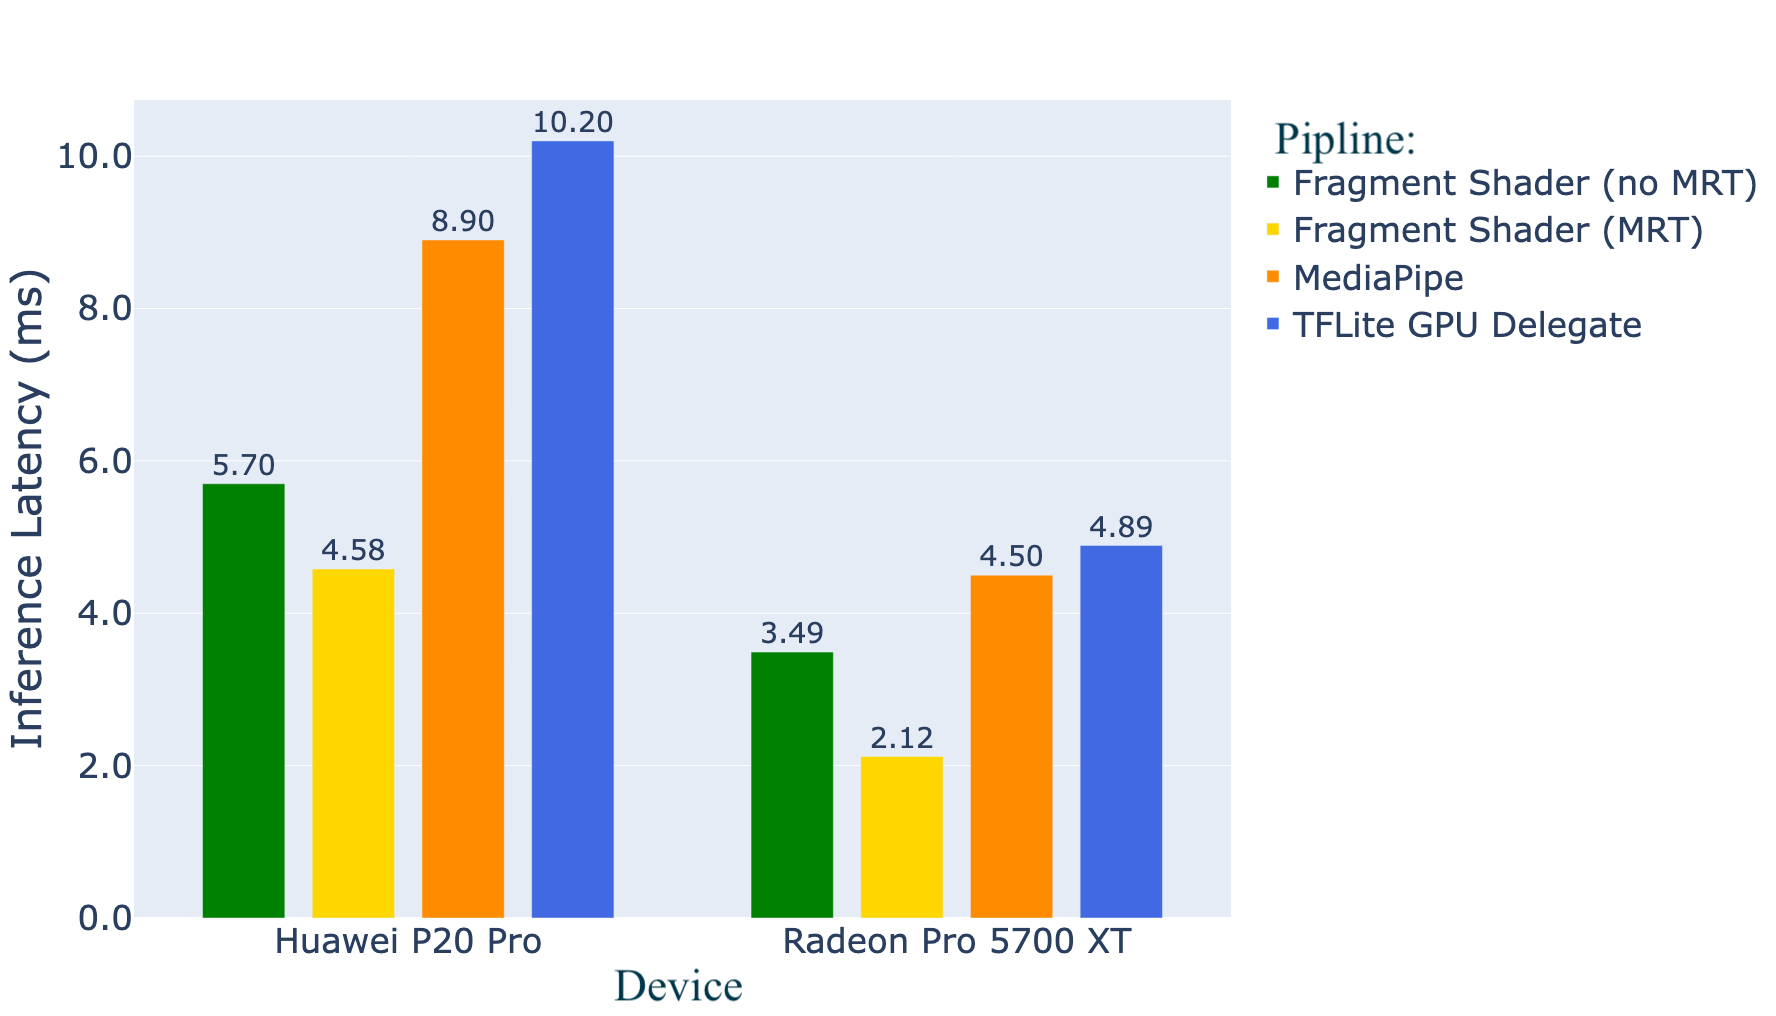
\includegraphics[width=\linewidth]{images/graphic.png}}
    \caption{Comparison of ESPCN [4] model inference latency on different GPUs and pipelines}
    \label{ris:ORTModelData}
\end{figure}
            
As demonstrated in Figure 1, the shader implementation (in both modes) exhibits a substantial advantage in terms of execution time in comparison to MediaPipe [3] and TFLite [1]. It is evident that on the Huawei P20 Pro, the pipelining on fragment shaders yielded an average latency of 5.3 milliseconds, whereas MediaPipe [3] and TFLite [1] exhibited respective averages of 8.9 and 10.2 milliseconds. The discrepancy is particularly evident in the desktop system, wherein the shader implementation exhibits latency ranging from 2.1 to 3.5 milliseconds, whereas MediaPipe [3] and TFLite [1] demonstrate latency exceeding 4 milliseconds.
            
The results obtained demonstrate that, with effective organisation of the computational graph of the model and the judicious selection of GPU-oriented primitives, the implemented pipelines can exhibit significantly superior performance in comparison to existing solutions without the necessity for third-party libraries or platform dependencies. The advantage is especially apparent in mobile inferencing, where response time is critical to ensure the quality of user experience in augmented reality and real-time computer vision tasks.

\section{Conclusion}
This paper presents a GPU-only pipeline to run the ESPCN [4] model on OpenGL [5] shaders without $CPU \xrightarrow{} GPU$ overhead. The developed pipeline demonstrates that fragment shaders can be effectively utilized for neural network inference. Due to the limited number of operations within the ESPCN network, the overheads associated with data transformation and transfer within the universal framework, and the subsequent return of results to the GPU pipeline are of considerable significance. The mean processing time for a frame in the implemented pipeline is more than twofold shorter than when using universal libraries, thus demonstrating the efficacy of the selected approach.

\begin{thebibliography}{00}
\bibitem{b1} TensorFlow Lite GPU Delegate. [Online]. Available: https://www.tensorflow.org/lite/performance/gpu
\bibitem{b2} PyTorch Foundation. (2025). PyTorch Mobile: End-to-end workflow from Training to Deployment for iOS and Android mobile devices [Online]. Available: https://pytorch.org/mobile/home
\bibitem{b3} MediaPipe Framework. [Online]. Available: https://mediapipe.dev
\bibitem{b4} Shi W. \textit{et al.}, Real-time single image and video super-resolution using an efficient sub-pixel convolutional neural network //Proceedings of the IEEE conference on computer vision and pattern recognition. – 2016. – P.1874-1883.
\bibitem{b5} Khronos Group. OpenGL Specifications. [Online]. Available: https://www.khronos.org/opengl/
\bibitem{b7} A. G. Howard \textit{et al.}, “MobileNets: Efficient Convolutional Neural Networks for Mobile Vision Applications,” \textit{arXiv preprint}, 2017.
\end{thebibliography}

\end{document}
